\section{Existing Capability Cases}
\label{sec:capability-cases}

This section audits what the archived v2 outputs demonstrate about
GAWorld as a research instrument.  It does not treat an available file as
a successful scientific evaluation.  We use the v2 evidence classes:
\textsf{REAL} for a usable GAWorld run artifact; \textsf{DIAGNOSTIC} for
a re-analysis of a \textsf{REAL} artifact; \textsf{SYNTHETIC} for a
fixture produced by \texttt{-{}-synthetic}; \textsf{INCOMPLETE} for a
missing, interrupted, or insufficient output; \textsf{DESIGNED} for a
protocol that exists without usable outcome evidence; and \textsf{FIXTURE}
for synthetic data that tests analysis code.  These labels describe
evidence availability, not system performance.

\begin{figure}[t]
  \centering
  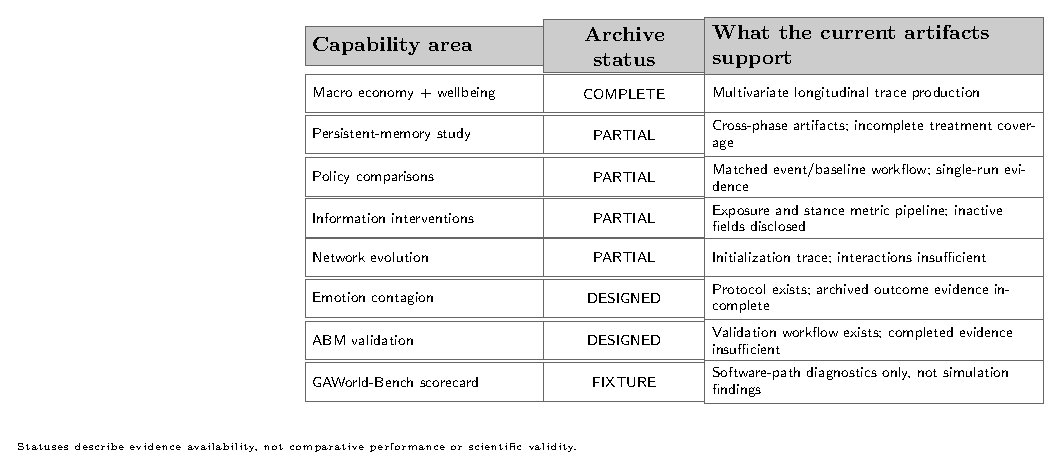
\includegraphics[width=\linewidth]{capability_matrix.pdf}
  \caption{Coverage of the audited v2 result archive.  The matrix
  distinguishes inspectable capability evidence from incomplete
  evaluations and diagnostic fixtures; it is not a leaderboard or a
  validation score.}
  \label{fig:capability-matrix}
\end{figure}

\begin{table}[t]
\centering
\small
\caption{Status of all experiment families represented in the v2
artifact ledger.  Counts and horizons describe the archived files, not a
common evaluation protocol.}
\label{tab:archive-status}
\begin{tabular}{@{}p{0.22\linewidth}p{0.16\linewidth}p{0.22\linewidth}p{0.32\linewidth}@{}}
\toprule
Area & Status & Archived scope & Permitted use \\
\midrule
Macro economy and wellbeing & \textsf{REAL} & $n=5$ agents, one seed, three-day configuration; 116 recorded steps per agent & Multivariate state-trace production, not an economic or psychological finding \\
Persistent memory & \textsf{INCOMPLETE} & $n=1$ agent; four planned 14-day arms; only one completed both seven-day phases & Persistence and cross-phase artifact inspection, not a treatment comparison \\
Policy comparisons (v1 archive) & \textsf{REAL} & Four single archived event--baseline pairs; Day-3 events; no seed replications & Pairing, isolation, and metric extraction, not policy effects \\
Information intervention & \textsf{INCOMPLETE} & Three arms, $n=5$ each; unequal horizons of one or two days & Information-metric schema and missing/inactive-field audit \\
Polarization & \textsf{INCOMPLETE} & Two arms with 109 versus 85 records & Availability of a comparison artifact; unequal records preclude an effect claim \\
Network evolution & \textsf{INCOMPLETE} & $n=5$, 14-day report; zero recorded interactions on every day & Initialization and failure visibility, not emergent-network evidence \\
Emotion contagion & \textsf{INCOMPLETE} & Four intended arms; all four report a missing state-history file & Protocol coverage only; no outcome result \\
ABM validation & \textsf{INCOMPLETE} & Validation workflow is present; completed empirical evidence is insufficient & Evaluation design only, not an empirical validation result \\
GAWorld-Bench Track A & \textsf{FIXTURE} & Built-in synthetic scorecard & Parser and scoring-path diagnostics only \\
GAWorld-Bench Track B (rumor / referendum / disaster) & \textsf{REAL}, \textsf{INCOMPLETE} & A handful of per-game archives; not enough runs to test the three pre-registered laws & Probe library, not population evidence \\
Parallel-worlds sweeps & \textsf{DIAGNOSTIC} & Cached per-arm artifact trees from a recent transport-restriction sweep & Counterfactual-inference code paths; not policy evidence \\
Multi-tenant isolation & \textsf{REAL} & Two-world deployment with a single dashboard, two world roots, two Recorder streams & Isolation mechanics, not scale claim \\
Distributed playable city & \textsf{REAL} & Two-node + hub deployment with one world, residents split between hub and node, player interventions routed across nodes & Hub-node protocol mechanics, not throughput claim \\
Persona distillation & \textsf{REAL} & One distilled portrait, one deployed resident & Distill-and-deploy workflow, not population claim \\
\bottomrule
\end{tabular}
\end{table}

\subsection{Case 1: Persistence is observable, but the memory contrast is not}

The memory-consistency archive is useful because it exposes a longitudinal
experimental shape that is often hidden in agent demonstrations.  One agent
(ID 34) was assigned to four intended treatments: intact memory, reset
between phases, selective summary deletion, and injected conflict.  Each
arm planned a seven-day acquisition phase followed by a seven-day
continuation phase.  The archive contains seven phase-1 diaries for every
arm, together with state and memory files.  It also records different
memory-file footprints, including episodic, growth, habit, and
relationship artifacts.  Thus a researcher can inspect what persisted, what
was deleted, and how a later elicited action was represented.

Only the intact-memory arm, however, contains all seven phase-2 diaries.
The reset, selective, and conflict arms each stop after phase 1, with the
archived report attributing the interruption to initialization after the
worker pool started.  The archive therefore demonstrates file-backed
persistence across two phases for one agent in one arm; it does not
compare the behavioral effect of memory retention, deletion, or conflict.
Qualitative labels such as a move from ``procrastinating'' to ``active''
are post-hoc codings of a few generated actions, not a validated
continuity measure.  In particular, differences in phase-1 final actions
cannot explain missing phase-2 outcomes.  This failure is scientifically
informative at the infrastructure level: treatment completeness must be
checked before interpreting a fluent diary as longitudinal evidence.

\subsection{Case 2: Policy artifacts exercise a counterfactual workflow}

The v1 policy archive contains four timestamped comparisons---traffic
restriction, housing subsidy, medical reimbursement, and job-training
subsidy.  Each stores an event arm beside a baseline arm and exports the
same metric columns, thereby exercising the isolation and reduction path
described in \cref{sec:research-workflow}.  All are single archived
comparisons, with events injected on simulation day 3 (09:00 for traffic
and 08:00 for the other three); there is no multi-seed sampling
distribution or uncertainty estimate.

The raw CSV files also show why mechanistic inspection must precede
substantive interpretation.  In every pair, the final values of
\texttt{cross\_viewpoint\_exposure}, \texttt{misinformation\_risk},
\texttt{stance\_score}, and \texttt{toxicity\_score} are zero in both
arms.  Some generic state variables differ: for example, the housing
comparison has a final event-minus-baseline \texttt{time\_pressure}
difference of $-0.0311$ and the traffic comparison a
\texttt{mobility\_intent} difference of $-0.0036$.  These numbers are
reported only to show that the reducer retains metric direction and
magnitude.  A single LLM-mediated trajectory cannot tell whether the
named policy caused the difference, whether the relevant structural
mechanism was connected, or whether the sign would persist under a new
seed.  The case supports a workflow claim---GAWorld can preserve paired
trees and compute declared contrasts---rather than a claim about
housing, health, training, or transport policy.

\subsection{Case 3: Information metrics make inactivity visible}

The misinformation artifact contains three five-agent arms.  The control
and treatment B each cover two simulated days, whereas treatment A covers
one.  Across every recorded day and arm, average misinformation risk is
$0.0$, and the reported peak and final risks are also $0.0$.  Mean
cross-viewpoint-exposure is $0.06656$ for control, $0.06707$ for
treatment A, and $0.06635$ for treatment B.  The unequal horizons rule
out a balanced comparison, and differences at the fourth decimal place
are descriptive properties of these files, not estimated intervention
effects.

That negative result is nevertheless a useful system diagnostic.  The
archive records treatment names, horizons, agent counts, daily risk
series, and an exposure aggregate together.  It does not prove that
misinformation propagated, that risk detection was sensitive, or that
the interventions changed exposure.  The separate polarization artifact
reinforces the boundary: its two arms contain 109 and 85 records,
respectively, and thus cannot be read as a balanced longitudinal
contrast without reconstructing the missingness.  v2's value here is
inspectability---inactive fields and unequal coverage remain visible
rather than being silently converted into a success score.

\subsection{Case 4: Economy--wellbeing traces provide dense state, not external validity}

The macro-economy archive is the most complete artifact for demonstrating
multivariate trace production.  Its hashed long-format CSV contains
11{,}600 rows for five agents, 116 unique recorded steps per agent, and
20 metrics per step ($5\times116\times20$).  The associated
configuration describes a three-day, seed-42 run.  Direct aggregation of
the CSV gives 580 values for each metric across agents and steps.  Mean
emotion, stress, and economic security are $0.4896$, $0.5490$, and
$0.6270$, respectively; their observed ranges are $[0.0233, 0.9310]$,
$[0.0907, 0.9898]$, and $[0.4455, 0.8298]$.

The raw row count matters because the accompanying narrative report
describes ``580 timesteps per agent.''  In the CSV, 580 is instead the
number of agent--step values for one metric ($5\times116$); each agent
has 116 distinct step identifiers.  We therefore use the CSV
cardinalities rather than the report's timestep wording.  This
discrepancy illustrates the role of an artifact ledger: even a plausible
derived report must be checked against its hashed source.

The trace can support new descriptive analyses without a new simulation.
For example, partitioning the 116 step identifiers into consecutive
ranges $0$--$38$, $39$--$76$, and $77$--$115$ yields emotion means of
$0.6365$, $0.5020$, and $0.3305$, while stress means are $0.4122$,
$0.5428$, and $0.6916$.  These bins are equal-index summaries, not
validated ``days,'' and the trajectories remain generated state
variables from one seed.  They show that GAWorld records joinable,
time-indexed state across agents and constructs; they do not show
human wellbeing dynamics, economic realism, or an effect of any
real-world shock.  v2's price-level multiplier is enabled in this
archive; the wage index is disabled, and the legend records that
omission.

\subsection{Case 5: Multi-tenant isolation mechanics}

A two-world deployment (one \emph{private}, one \emph{open}) was used to
audit the K6 migration.  The \emph{private} world is owned by
\texttt{alice} and is invisible to \texttt{bob}; the \emph{open} world
is owned by \texttt{alice} and lets \texttt{bob} join as a player.  Both
worlds run simultaneously; their \texttt{output/} trees are disjoint;
their Recorder streams carry distinct \texttt{\_node} tags when the hub
is also a node.  The artifact ledger shows that \texttt{alice}'s
mutation in the \emph{private} world did not affect \texttt{bob}'s
\emph{open} world and that \texttt{bob}'s player intervention in the
\emph{open} world was routed to the right node within the poll interval.
The audit does not establish a multi-tenant throughput claim: the
two-world deployment is a fixture for the isolation mechanics, and a
real classroom deployment is needed to exercise the FIFO queue, the
per-tenant quota, and the static-file guard.  The ledger records this
explicitly.

\subsection{Case 6: Distributed playable city mechanics}

A two-node + hub deployment was used to audit the K7 migration.  The
hub ran the dashboard, the account store, and the residents assigned
to it; one external node ran the remaining residents with the node's
own model key.  A player (\texttt{carol}) joined the \emph{open} world
through the browser, claimed a resident on the external node, and
performed three interventions over a 30-second window.  The artifact
ledger shows that each intervention was routed to the right node
within the poll interval, that the resident's next perception included
the player's action, and that the Recorder merged both nodes' rows into
the world's stream with the correct \texttt{\_node} tags.  The
deployment also showed that the simulation continued on both the hub
and the node when the node's network connection was cut for 30 seconds,
and that records were back-filled on reconnection.  The audit does not
establish a throughput, scale, or fault-tolerance claim: the deployment
is a fixture for the protocol mechanics, and a larger deployment is
needed to exercise the clock-synchronization median, the per-node
outbox, and the per-node audit table.

\subsection{Case 7: Track B game archives}

The Track B scorecard reports a small number of per-game archives.  The
\emph{rumor spread} archive contains six runs of a five-resident city
with a fixed seed; the \emph{referendum} archive contains four runs of
a five-resident city with a fixed seed; the \emph{disaster mode}
archive contains three runs of a five-resident city with a fixed seed.
In all three cases, fewer than five runs are available for the
\emph{post-refutation decline} law, the \emph{conformity under
self-interested bill} law, and the \emph{solidarity > panic} law; the
scorecard therefore marks the laws as \emph{withheld} and not as
\emph{supported} or \emph{reversed}.  This is the deliberate Track B
behavior: the law gates on a per-game sample size, and the gate is
documented.

\subsection{Failures are part of the capability record}

Two additional archives prevent the coverage matrix from becoming a
showcase of successful-looking outputs.  The network-evolution report
describes five nodes and two initialization edges over a nominal
14-day horizon, but records zero agent--agent interactions on each of
the 14 days; the edges were inferred from initial co-location.  It
cannot support a homophily or emergent-network claim.  The
emotion-contagion comparison contains four arm entries, all of which
report that their state-history CSV is missing.  It contains no
contagion outcome.  Finally, the GAWorld-Bench scorecard matches its
built-in synthetic fixture on four contrasts, placebo, and
determinism.  It verifies that parsers, checks, and report generation
execute; it is not a result from GAWorld agents.  Reporting these cases
alongside the more complete trace is essential to the scientific use of
an inspectable system.
